\documentclass[11pt, a4paper, oneside, twocolumn, dvipdfmx]{jsarticle}
\usepackage{url}
\usepackage{graphicx}
\usepackage{geometry}
\geometry{top=1cm,  bottom=2cm, left=1.5cm, right=1.5cm}
\pagestyle{empty}
\usepackage{amsmath}
\usepackage{amssymb}
\usepackage{tikz}
\usetikzlibrary{intersections,calc,arrows.meta}
\setlength{\intextsep}{10pt}
\setlength{\textfloatsep}{10pt}

\newcommand{\simname}{SimSym}
\newcommand{\simnamealt}{Simulation with Symbols}

\title{物理学の学習のためのプログラマブルな
\\シミュレータと環境の提案}

\author{東京工業大学 情報理工学院 数理・計算科学系\\18B04657 木内康介\\指導教員 増原英彦教授}

\date{}

\begin{document}
\maketitle

\section{はじめに} \label{intro}
高等学校における物理学の授業において、実験は重要である。Holubova~\cite{holubova_2019}は、実験室での作業は理論的な概念を検証する最も重要な方法であり、生徒は実験を通してどのような現象が起きるかを確認することができると述べている。

しかし実際は、生徒全員が実験を経験しているわけではない。力学分野において最も基本的な「運動の法則」に関する実験経験は、2014年の調査時点で60\%にしか満たない~\cite{2015KJ00010038066}。
理由としては、実験用の装置の準備や測定が難しいことや、実験を行うのに時間を要することが考えられる。

そこで実験の代替として近年利用されているのが、物理実験のシミュレータである。シミュレータを用いることで、実験と同様の学習効果を得ることができる~\cite{ajredini_real_2014}。

しかし、実際に生徒が解く問題の解答過程と既存のシミュレータの間には、確認できる情報にギャップがある。高等学校で扱う物理の問題では図~\ref{symbol_based}のように方程式の計算を要求される。一方、例えばPhET~\cite{perkins_phet_2006} は、図~\ref{numeral_based}のように速度や質量、位置のような物理量を数値で与えることで指定された運動が描画される。そのため、可視化された運動がどのような方程式によるものなのか確認することができない。
% また、既存のシミュレータは設定されたシチュエーションの中でパラメータを変更できるにすぎず、学習者が解いている問題の設定と一致するシミュレーションが常に存在するわけではない。

\begin{figure}[b]
% 静止している質量 $m$ の物体に大きさ $F$ の力をかけ続ける。 $t$ 秒後の速度の大きさを求めよ。
% \begin{align}
%   \left\{
%   \begin{aligned}
%     ma &= F & (1)\\
%     v &= at & (2)
%   \end{aligned}
%   \right. \nonumber
% \end{align}
% (1)より、$a = \dfrac{F}{m}$ \quad (2)に代入して、$v = \dfrac{F}{m}t$
% \centering
% 答え: $\dfrac{F}{m}t$

\noindent\rule{\linewidth}{0.4pt}

\small{\textbf{(問題)} 静止している質量 $m$ の物体に大きさ $F$ の力をかけ続ける。$t$ 秒後の速さを求めよ。}

\small{\textbf{(解答)} 物体の加速度を $a$ とする。運動方程式より $ma~=~F$ $\therefore~a~=~\dfrac{F}{m}$ 。等加速度運動の公式より $v~=~at~=~\dfrac{F}{m}t$\\
答え: $\dfrac{F}{m}t$}

\caption{方程式の計算例} \label{symbol_based}
\end{figure}

\begin{figure}[thb]
\centering
\includegraphics*[width=0.9\linewidth]{figure/PhET_example.png}
\caption{PhET のシミュレーション例} \label{numeral_based}
\end{figure}

そこで本研究では、物理系を定義できるシミュレータである \simname~(\simnamealt) を提案する。学習者は \simname で系内の物体をそのパラメータとともに定義し、その物体の運動を表す方程式を立式する。\simname は、次元の異なる物理量の和などの不正な方程式を警告するなど、学習者が正しい物理系を作成するための補助を行う。シミュレーションを実行すると、定義した物理系に基づいて数値計算がなされ、物体の運動が可視化される。[TODO: 教師役の話]

既存のシミュレータは教師役が物理系を全て定義し、学習者はパラメータを指定するだけである。[TODO: SimSym による学習効果のはなし]

% これにより、学習者は解いている問題の設定と一致するシミュレーションを作ることができる。

なお、\simname は大部分が未実装であるが、\ref{sec2}節で説明するアイデアは\ref{sec3}節に記す方針で実装が可能であると考えている。

\section{\simname} \label{sec2}

学習者は、\simname で以下の操作によって物理系を定義し、シミュレーションを実行することができる:

\begin{enumerate}
\item \textbf{物体の作成}: 学習者が物体名を入力すると、\simname はその物体に紐付いた物理量に対応する次元付き変数($m_A\mathrm{[M]}, x_A\mathrm{[L]}$ など)を生成する。
\item \textbf{方程式の立式}: 学習者は、1.で生成された変数を使って方程式を立式する。この際、次元付き変数は自由に追加することができる。なお、時刻を表す変数 $t\mathrm{[T]}$ や重力加速度 $g\mathrm{[L/T^2]}$ などの物理定数は用意されている。また、不正な次元の方程式は警告される。
% \item \textbf{物体と方程式の紐付け}: 学習者は方程式を物体のフィールドにドラッグすることで、そのフィールドに方程式を紐付け、フィールドの値を方程式に数値を代入した結果にすることができる。方程式とフィールドの次元が一致していない場合、紐付けることはできない。
\item \textbf{シミュレーションの実行}: 学習者が観測したい変数を指定すると、時刻 $t$ が変化しながら各方程式が計算され、指定した変数に対応した物理量が可視化される。なお、シミュレーションの実行のために必要な変数には初期値を与える必要がある。
\end{enumerate}

[TODO: Paneの話]

物体の名前を入力し物体作成ボタンを押すと、

以下では具体例を見ていく。図~\ref{simsym_fig1}は、\simname 上で斜方投射を表現した例である。この例ではy座標に紐付けている方程式が $v_{0y}t - \frac{gt^2}{2}$ となっているため、シミュレーションを再生すると図~\ref{correct}のような軌道を描く。ここで、速度の次元を持つ $gt$ という方程式はy座標に紐付けることができない。また、$(\text{位置}) - (\text{速度})$ という形になっている $v_{0y}t - gt$ という方程式を作成しようとすると、次元が一致していないため警告され、定義できない。

\begin{figure}[htb]
  \centering
  \includegraphics*[width=0.9\linewidth]{work/slide_img4-crop.pdf}
  \caption{\simname 上で斜方投射を表現した例} \label{simsym_fig1}
\end{figure}

\begin{figure}[htb]
\centering
% \begin{minipage}{0.4\linewidth}
\begin{minipage}{0.8\linewidth}
\centering
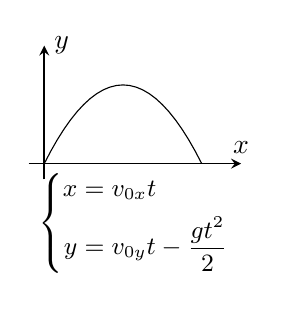
\begin{tikzpicture}
\draw[->,>=stealth,semithick](-0.2,0)--(2.5,0)node[above]{$x$}node[anchor=north east]{$\small{\left\{ \begin{aligned} x &= v_{0x}t \\ y &= v_{0y}t-\frac{gt^2}{2} \end{aligned} \right.}$};
\draw[->,>=stealth,semithick](0,-0.2)--(0,1.5)node[right]{$y$};
\draw[domain=0:2]plot(\x,{-1 * pow(\x-1, 2) + 1});
\end{tikzpicture}
\caption{斜方投射の軌道} \label{correct}
\end{minipage}
% \begin{minipage}{0.4\linewidth}
% \centering
% \begin{tikzpicture}
% \draw[->,>=stealth,semithick](-0.2,0)--(2.5,0)node[above]{$x$}node[anchor=north east]{$\small{\left\{ \begin{aligned} x &= v_{0x}t \\ y &= v_{0y}t+\frac{gt^2}{2} \end{aligned} \right.}$};
% \draw[->,>=stealth,semithick](0,-0.2)--(0,2.5)node[right]{$y$};
% \draw[domain=0:2]plot(\x, {(pow(\x+1, 2) - 1) / 4});
% \end{tikzpicture}
% \caption{誤った軌道} \label{wrong}
% \end{minipage}
\end{figure}

\section{実装の方針} \label{sec3}
フロントエンドに lively.next[TODO: 引用]\footnote{\url{https://lively-next.org}} を、方程式の処理と数値計算に SymPy~\cite{meurer_sympy_2017} を用い、JavaScript で実装する。lively.next は、GUIアプリケーションを作成・実行するためのWebプログラミング環境である。学習者が物体や方程式を定義する画面とシミュレーションを表示する画面を lively.next で作成する。SymPy は、記号計算のための Python ライブラリであり、Pyodide~\footnote{\url{https://pyodide.org/en/stable/}} を用いることで WebAssembly に変換し、ブラウザで実行する。\simname は、入力された物理量や方程式を SymPy オブジェクトに変換することで、数値計算を可能にする。[TODO: 具体的にどのように計算し可視化するか]

%その結果に基づき、 lively.next で表示する。

% \subsection{Pyodide}
% Pyodide は、WebAssembly で実装された CPython 処理系である。ブラウザ上で Python 並びにいくつかのパッケージを実行することができる。これを用いて、lively.next から SymPy を呼び出して計算することをブラウザ上だけで完結させることができる。

\section{まとめと課題}
本研究では、物理系を定義できるシミュレータ \simname を提案した。学習者は\simname を用いることで
% 学習者は解いている問題の設定と一致するシミュレーションを作り、
自身が定義した物理系の運動と現実の運動との対応を視覚的に確認することができる。[TODO: SimSymによる学習効果のはなし]。

今後の課題は、\simname の教育効果の評価である。評価手法として、Hake~\cite{hake_1998}が導入した normalized gain を用いた実験を検討する。

\bibliographystyle{junsrt}
\tiny{\bibliography{thesis}}

\end{document}